%%-*- mode: LaTeX; mode: FlySpell; -*-

\documentclass{elsarticle}

\usepackage{amssymb,amsmath}

\usepackage{graphicx}
\usepackage{zed-csp}
%\usepackage{csp}
%\usepackage{algorithm}
%\usepackage{algpseudocode}
\usepackage{float}
\usepackage{url}
\usepackage{cite}
\usepackage{tabularx}
%\usepackage{cases}

% The line below was added as a workaround for spacing ``f'' in mathit. \mathit can now be replaced by \Lmathit to get better spacing. 
\DeclareMathAlphabet{\Lmathit}{\encodingdefault}{\familydefault}{m}{it}

\interdisplaylinepenalty=2500

\newfloat{algorithm}{tbp}{lop}
\floatstyle{ruled}

\newtheorem{lemma}{Lemma}%
\newtheorem{definition}{Definition}%
\newtheorem{conjecture}{Conjecture}%
\newtheorem{theorem}{Theorem}%
\newtheorem{proposition}[theorem]{Proposition}

% include if zed-csp is not included.
% \newcommand{\hide}{\setminus}
% \newcommand{\spot}{\bullet}

%include if zed-csp IS included.
\renewcommand{\inv}{\mathit{inval}}
%otherwise
%\newcommand{\inv}{\mathit{inval}}

\newcommand{\prov}{\mathit{prov}}
\newcommand{\dep}{\mathit{dep}}
\newcommand{\pr}{\mathit{pr}}
\newcommand{\obf}{\mathit{abs}}
\newcommand{\pol}{\mathit{pol}}

\newcommand{\pg}{\mathit{PG}}
\newcommand{\en}{\mathit{En}}
\newcommand{\act}{\mathit{Act}}
\newcommand{\ag}{\mathit{Ag}}

\newcommand{\used}{\Lmathit{used}}
\newcommand{\wgby}{\Lmathit{genBy}}
\newcommand{\influence}{\Lmathit{wasInfluencedBy}}
\newcommand{\wdf}{\Lmathit{wasDerivedFrom}}
\newcommand{\waw}{\Lmathit{waw}}
\newcommand{\attrTo}{\Lmathit{wat}}
\newcommand{\wat}{\Lmathit{wat}}
\newcommand{\delegate}{\Lmathit{abo}}
\newcommand{\wasInfBy}{\Lmathit{wasInformedBy}}
\newcommand{\start}{\Lmathit{start}}
\newcommand{\ed}{\Lmathit{end}}


\newcommand{\Ev}{\mathit{Ev}}
\newcommand{\preorder}{\preceq}

\newcommand{\evmap}{\mathit{evmap}}


\newcommand{\node}{\mathit{Node}}
\newcommand{\type}{\mathit{type}}
\newcommand{\elabel}{\mathit{label}}

\newcommand{\guEA}{\pg_{gu/ea}}  % gen-usage over enties, activities
\newcommand{\guiEA}{\pg_{gui/ea}}
\newcommand{\guaEAG}{\pg_{gu+/eaAg}}  % gen-usage and more over enties, activities plus Agents

%% operators
\newcommand{\group}{\mathit{Group}}
\newcommand{\aggroup}{\mathit{agGroup}}
\newcommand{\sgroup}{\mathit{Group_{str}}}
\newcommand{\clos}{\mathit{pclos}}
\newcommand{\repl}{\mathit{replace}}
\newcommand{\agrepl}{\mathit{agreplace}}
\newcommand{\rewire}{\mathit{rewire}}
\newcommand{\extend}{\mathit{extend}}
\newcommand{\pclos}{\mathit{pclos}}
\newcommand{\rem}{\mathit{remove}}
\newcommand{\agremove}{\mathit{AgRemove}}
\newcommand{\orphanremove}{\mathit{OrphanRemove}}
\newcommand{\allorphanremove}{\mathit{AllOrphanRemove}}
\newcommand{\remIsolated}{\mathit{remIsolated}}

\newcommand{\dclos}{\mathit{dclos}}

\newcommand{\POL}{\mathit{\cal P}}

%\newcommand{\mnote}[1] {\marginpar{\scriptsize \raggedright #1 }}
\newcommand{\mnote}[1] {  \framebox{\begin{minipage}[t]{0.9\linewidth}
 \scriptsize \raggedright #1 \normalsize
    \end{minipage}
 }}

\newenvironment{mydrop}{\begin{array}[t]{@{}l@{}}}{\end{array}}%



\usepackage{color}
\usepackage{pdfpages}
\usepackage{ifthen}
\newcommand{\showColour}{yes} % {yes}
\newcommand{\showComments}{yes} % {yes}
\newcommand{\note}[2]{\ifthenelse{\equal{\showColour}{yes}}{\textcolor{#1}{#2}}{#2}}
\newcommand{\jwb}[1]{\note{blue}{#1}}

\newcommand{\paolo}[1]{\note{magenta}{#1}}


\newcommand{\com}[2]{\ifthenelse{\equal{\showComments}{yes}}{\textcolor{#1}{#2}}{}}
\newcommand{\comment}[1]{\com{red}{#1}}



\begin{document}

\title{Blur And Collapse}


\author[ncl]{P. ~Missier\corref{cor1}}
\ead{Paolo.Missier@newcastle.ac.uk}

\author[cov]{J. ~Bryans\corref{cor2}}
\ead{Jeremy.Bryans@coventry.ac.uk}


\address[ncl]{School of Computing Science, Newcastle University, UK}
\address[cov]{Institute for Future Transport and Cities, Coventry University, UK}

\cortext[cor1]{Principal Corresponding Author}
\cortext[cor2]{Corresponding Author}

%\markboth{IEEE Transaction on Knowledge and Data Engineering,~Vol.~X, No.~Y, DATE}%
%{Shell \MakeLowercase{\textit{et al.}}: happy}


\begin{abstract}

\end{abstract}

\begin{keyword}
Provenance \sep Provenance metadata \sep provenance abstraction 
\end{keyword}

\maketitle

\section{Introduction and motivation}

\mnote{Running examples:  we may need two/three, one for each operator.
	
	PM: suggest picking p-graphs that are plausible when viewed as the trace of a program, ie using abstract function names for activities.
}
	
\mnote{main contributions:
	\begin{itemize}
	\item three graph rewriting operators for abstracting over provenance graphs, \jwb{two versions of blur, collapse, two versions of sibling collapse)}
          formalised and with proof that the rewriting preserves PROV validity
		\item algebraic properties of the operators (commutative??)
		\item small PROV extension to introduce new relationships when the existing ones are generalised i.e. to ``influence'', that is the new relationship types qualify ``influence''
               \item use Janetta's tool to show these available in an implementation
                  \item (AMBITION) demonstrate these useful as comprehension tools (so not obfuscation..) to the urban observatory as alternate interfaces to their data for the general public and experts. 
%		\item demonstration of how the operators support a variety of abstraction policies and how we cna use a variety of graph metrics to measure the effect of applying a specific policy to a graph
%		\item empirical evaluation of the rewriting i.e. using (1) a variety of synthetic graphs, generated using ProvGen, (2) a variety of policies chosen as representative examples and (3) a variety of provenance network metrics
 	\end{itemize}
	
}
	
\section{Background on PROV}

%%%%%%%%%%%%
%%
%%%%%%%%%%%%

\section{Background}
\label{sec:prov-background}

\subsection{Core PROV model} \label{sec:prov-core}

We now introduce the core elements of the PROV model, which forms the basis for the grouping operator.
%
We maintain a dual view of provenance, both as a relational model (with binary relations) and as a graph model. Viewed as a relational model, PROV includes three types of elements: Entities ($\en$), Activities ($\act$), and Agents ($\ag$), and several types of relations amongst them. 
In line with the description in~\citep{w3c-prov-dm} (Section 2), PROV is defined by the following core relations, with common abbreviations in brackets. 

\begin{eqnarray*}
Used~~(\used)  & \subseteq & \act \times \en \\
WasGeneratedBy~~(\wgby) & \subseteq  & \en \times \act \\
WasDerivedFrom~~(\wdf) & \subseteq   & \en \times \en \\
WasInvalidatedBy~~(\inv) &  \subseteq &  \en \times \act \\
WasAssociatedWith~~(\waw) & \subseteq & \act \times \ag \\
ActedOnBehalfOg~~(\delegate) & \subseteq & \ag \times \ag \\ 
WasAttributedTo~~(\attrTo) & \subseteq & \en \times \ag \\
WasInformedBy~~(\wasInfBy) & \subseteq & \act \times \act
\end{eqnarray*}


\begin{figure}
\centering
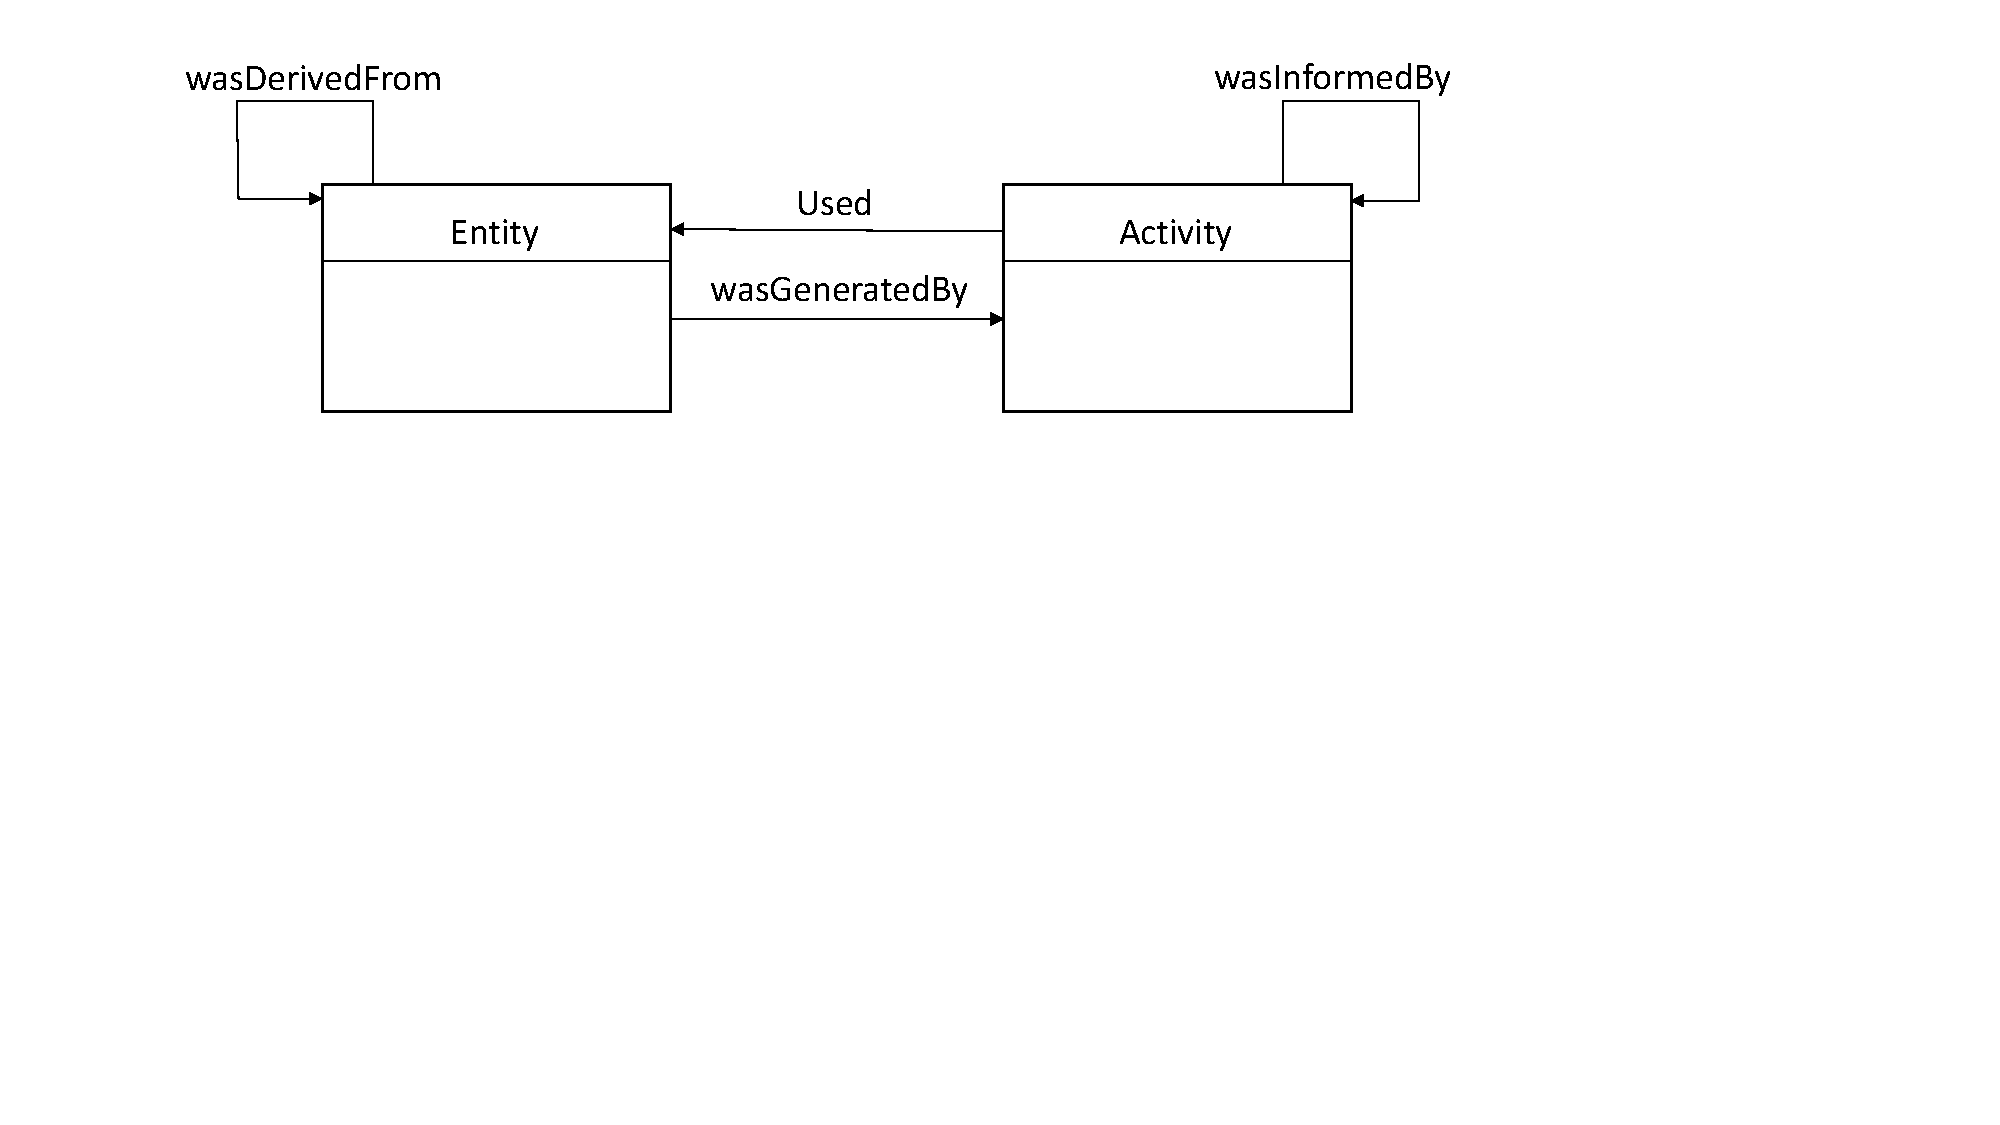
\includegraphics[scale=.45]{figures/prov-essentials.pdf} 
\caption{Core elements of the PROV model, adapted from~\citep{w3c-prov-dm}}
\label{fig:prov-core}
\end{figure}

%\subsection{Bipartite PROV: $\guEA$}  \label{sec:prov-guea}
These are summarized in Fig.~\ref{fig:prov-core}.
%

\jwbtwo{In this paper} we are going to restrict ourselves to an even simpler model, consisting only of $\en$, $\act$, and relations $\used$ and $\wgby$.
% Agents and the relations that involve them are introduced in Sec.~\ref{sec:agents-abstraction}.
%
Further extensions to the additional relations --- $\wdf$ and $\wasInfBy$ --- are straightforward and are not considered in detail.

%
An instance  of the model is a provenance document $D$, consisting of sets $en \in \en$ and $act \in \act$ of symbols, and sets of relation instances $\{ \wgby(e,a)  | e \in \en, a \in \act \} \cup   \{ \used(a,e)  | e \in \en, a \in \act\}$. 

%
As these relations are binary, we view $D$ as a digraph $G=(V,E)$, where $V= \en \cup \act$, and each relation instance maps to a labelled directed edge. By convention, we orient these edges from right to left, to denote that the relation ``points back to the past''. Thus:
$a \xleftarrow{\wgby} e \in E$ iff $\wgby(e,a) \in D$, and $e \xleftarrow{\used} a \in E$ iff $\used(a,e) \in D$.
%
We denote the label associated to edge $(v_i, v_j)$ as $\elabel(v_i,v_j)$. 

%
Note that, by definition of the relations, $G$ is a bipartite graph.
We denote the set of all such graphs by $\guEA$, to indicate that they only contain $\en$ and $\act$ nodes, and $\wgby$ and $\used$ edges.
Fig.~\ref{fig:baseline-ug-ae} portrays a simple $\guEA$ graph that we will be using as a running example. %\comment{This sentence isn't true. Fig 5 isn't the same as fig 6. Fig 6 = Fig 7,  but then Fig 8 = Fig 5. }

 %In Sec.~\ref{sec:agents-abstraction} we are going to extend this set to include agents as well as additional relations.

%\comment{Old version is above, new below}

\begin{figure}
\centering
%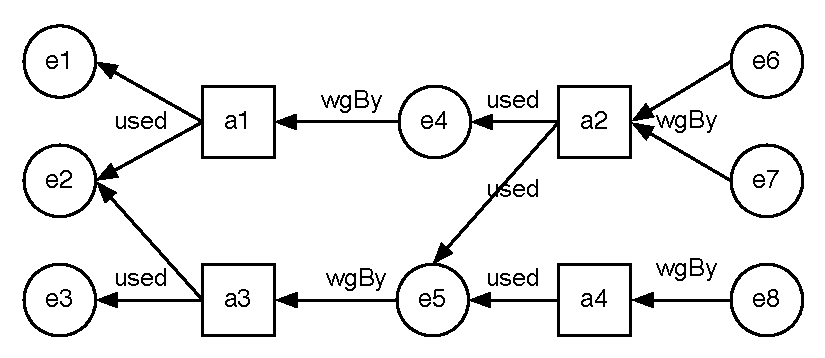
\includegraphics[scale=.6]{figures/baseline-ug-ae.pdf} 
%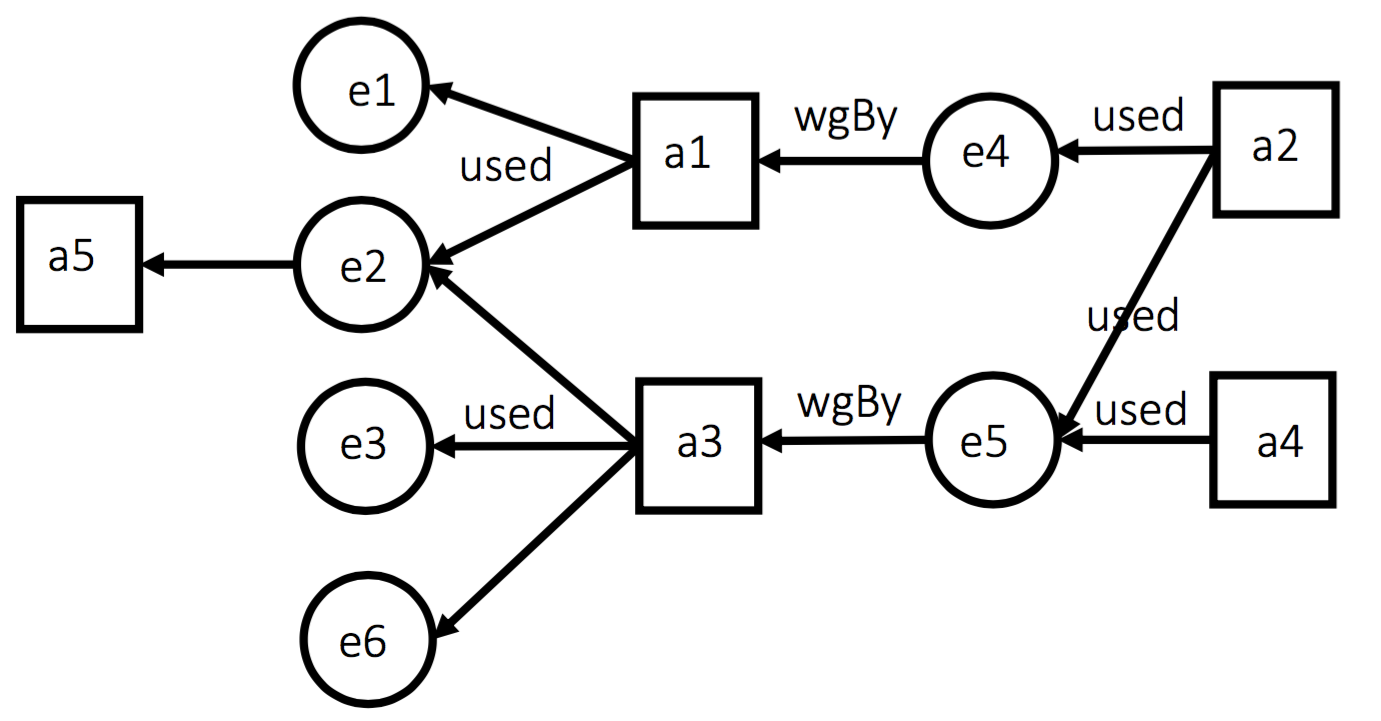
\includegraphics[scale=.15]{reworked-fig5.png} 
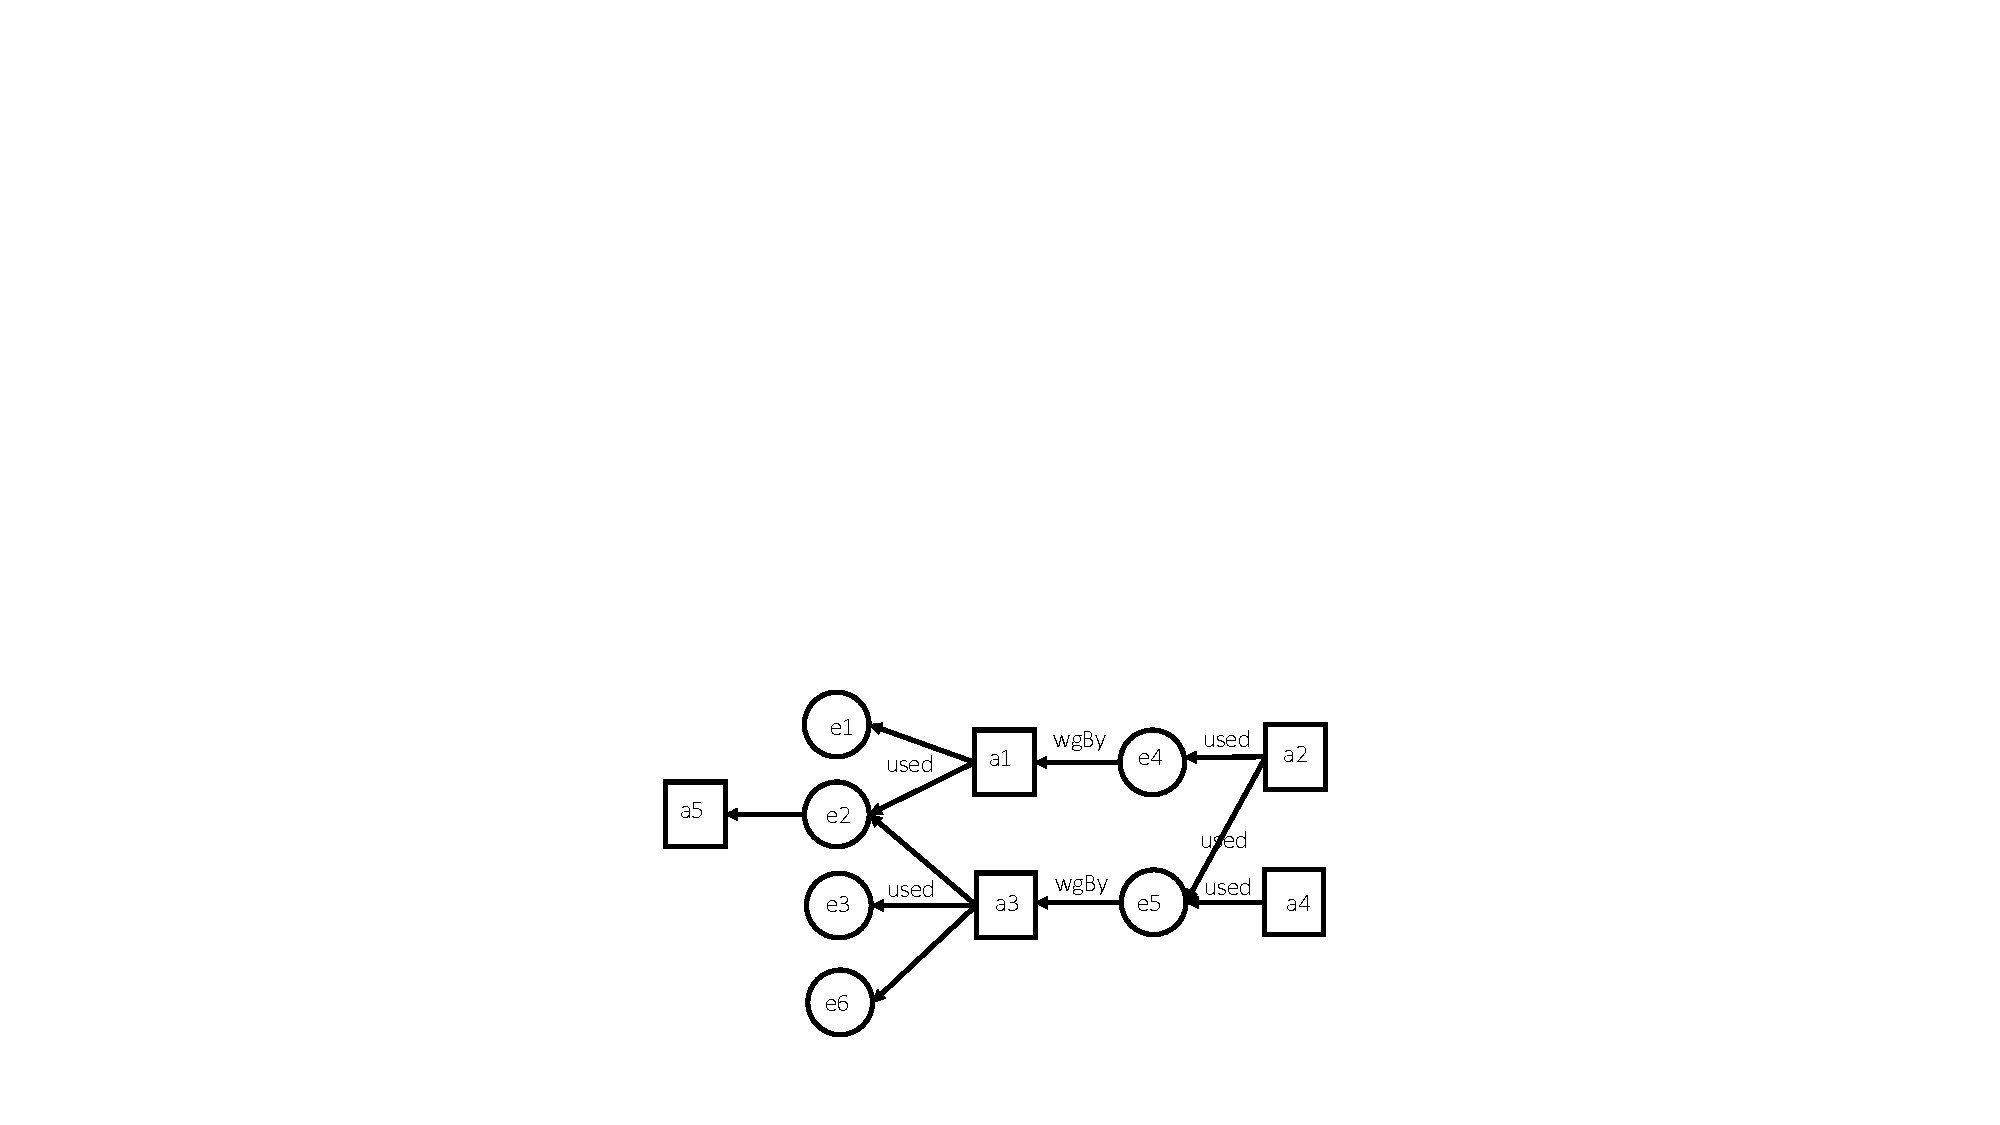
\includegraphics[scale=.6]{reworked-fig5.pdf} 
\caption{$\guEA$ provenance graph used as a running example to illustrate abstraction by grouping.}  \label{fig:baseline-ug-ae}
\end{figure}

\subsection{Events in $\guEA$}  \label{sec:prov-events}

\label{sec:events}

Central to PROV is the notion that provenance is marked by events. A partial order is defined over events, so that it may or may not be possible to establish whether or not one event precedes another. 
%
Events occur instantaneously, and they mark the lifetime boundaries of Entities (generation, invalidation), Activities (start, end), and Agents (start, end), as well as some of the interactions amongst those elements. These include the generation and usage of an entity by an activity, attribution of an entity to an agent, and more. More specifically, the PROV-CONSTRAINTS document~\citep{w3c-prov-constraints} defines the following types of events (quoted verbatim from Section 2.2):

\begin{itemize} %
	\item\textbf{An activity start event} is the instantaneous event that marks the instant an activity starts.
	
	\item\textbf{An activity end event} is the instantaneous event that marks the instant an activity ends.
	
	\item\textbf{An entity generation event} is the instantaneous event that marks the final instant of an entity's creation timespan, after which it is available for use. The entity did not exist before this event.
	
	\item\textbf{An entity usage event}  is the instantaneous event that marks the first instant of an entity's consumption timespan by an activity. The described usage had not started before this instant, although the activity could potentially have used the same entity at a different time.
	
	\item\textbf{An entity invalidation event} is the instantaneous event that marks the initial instant of the destruction, invalidation, or cessation of an entity, after which the entity is no longer available for use. The entity no longer exists after this event.
	
\end{itemize}
%\end{description}

We formally express events by introducing a set $\Ev$ of event symbols, with a pre-order\footnote{Recall that a pre-order is a binary relation with reflexivity and transitivity, but no symmetry or anti-symmetry.} $\preorder ~~\subset \Ev \times \Ev$, and the following set of partial functions that associate events to elements and relations in a provenance instance:
\begin{align*}
start: \act \rightarrow \Ev \\
end: \act \rightarrow \Ev \\
ev: \wgby \cup \used \cup \inv \rightarrow \Ev
\end{align*}	
As an example, in the graph of Fig.~\ref{fig:baseline-ug-ae} the generation relation $\wgby(e_4, a_1)$ has an associated generation event $ev(\wgby(e_4, a_1))$, whilst $a_1$ has start and / or end events, written $start(a_1)$ and $end(a_1)$, respectively. Similarly, usage of $e_4$ by $a_2$ is marked by event $ev(\used(a_2, e_4))$. Finally, if $e_4$ had been invalidated by some $a$ (not in the figure), this would be represented by an invalidation event $ev(\inv(e_4,a))$.

Temporal constraints involving events, and expressed by means of their pre-order relation $\preorder$, play a key role in the definition of \textit{valid} provenance instances, as described next.

\subsection{Constraints and valid $\guEA$ graphs}
\label{sec:prov-constraints}

%As mentioned earlier, our goal in this work is to define transformations of a valid PROV instance into new valid instance, whilst providing obfuscation by abstracting out some of its details. 
Validity of a PROV document is defined in terms of a set of constraints, as stated in the PROV-CONSTRAINTS document~\citep{w3c-prov-constraints}.
%
For instance, Constraint 55 states that the Entities and Activities are disjoint:  $\en \cap \act = \emptyset$.
Thus, a document $D$ that contains both statements (1) $a_1 \used~e_1$ and (2) $e_1 \used ~a_1$ cannot be valid, because by definition% of $\used$ given earlier,
 (1) entails  $e_1 \in \en$, $a_1 \in \act$, while (2) entails $a_1 \in \en$, $e_1 \in \act$, violating the constraint.
%
Note that disjointness constraint 55 entails that $\guEA$ graphs are bipartite.

In this paper we are mainly concerned with temporal constraints, which apply to $\guEA$ instances and determine the admissible partial ordering of the event types introduced in the previous section.
With reference to a graph $\pg$, these are (including constraint (55) above, and using the original numbering in~\citep{w3c-prov-constraints})

\begin{itemize}
	
	\item\textbf{C1: entity-activity-disjoint (Constraint 55):} \[\en \cap \act = \emptyset\]
	
	\item\textbf{C2: generation-generation-ordering (Constraint 39):}  If an entity is generated by more than one activity, then the generation events must all be simultaneous.
	
	Let 
	$gen_1 = ev(\wgby(e, a_1))$, $gen_2 = ev(\wgby(e, a_2)) \in \pg$. Then  \[gen_1  \preorder  gen_2, \quad gen_2 \preorder gen_1\] must hold.
	
	\item\textbf{C3: generation-precedes-usage(Constraint 37):} A generation event for an entity must precede any usage event for that entity.
	%
	For any $a \in \act$ such that $\used(a,e) \in \pg$, \[	ev(\wgby(e, a)) \preorder ev(\used(a,e))\] must hold.
	
	\item\textbf{C4: generation-precedes-invalidation (Constraint 36):} The generation event (or, more accurately, the set of simultaneous generation events) for an entity must precede the invalidation event.
	
	For any $a,a' \in \act$ such that $\wgby(e, a))$, $\inv(e,a') \in \pg$ :
	\[ ev(\wgby(e, a)) \preorder ev(\inv(e,a')) \]
	
	\item\textbf{C5: usage-precedes-invalidation (Constraint 38):} Any usage event for an entity must precede the invalidation event.
%	
	For any $a,a' \in \act$ such that $\used(a,e))$, $\inv(e,a') \in \pg$ :
	\[ ev(\used(a,e)) \preorder ev(\inv(e,a')) \]
	
	\item\textbf{C6: usage-within-activity (Constraint 33):} Any usage of $e$ by $a$ cannot precede the start of $a$ and must precede the end of $a$. For any $e\in \en, a \in \act$ such that $\used(a,e) \in \pg$:
	\[start(a) \preorder ev(\used(a,e))   \preorder end(a)\]
	
	\item\textbf{C7: generation-within-activity (Constraint 34):} The generation of $e$ by $a$ cannot precede the start of $a$ and must precede the end of $a$.
	Let $\wgby(e,a) \in \pg$:
	\[ start(a) \preorder ev(\wgby(e,a))  \preorder end(a)\]
	
	\item\textbf{C8: invalidation-invalidation-ordering (Constraint 40):}	If an entity is invalidated by more than one activity, the events must all be simultaneous. \jwbtwo{If $\inv(e,a_1), \inv(e,a_2) \in \pg$, then }
	  \begin{align*}
          &\jwbtwo{ev(\inv(e,a_1)) \preorder  ev(\inv(e,a_2)) ~~\mathrm{and}} \\
          &\jwbtwo{ev(\inv(e,a_2)) \preorder  ev(\inv(e,a_1))}
          \end{align*}
\jwbtwo{must hold.}

\end{itemize}

Additional relevant constraints state that multiple start (resp. end, invalidation) events must all be simultaneous, and that the start event of an activity must precede the end event for that activity.
\\

\begin{definition}[Validity]
 A graph $G \in \guEA$ is valid iff it satisfies constraints C1-C8.
	\label{def:valid-guea}
\end{definition}

%\comment{should finish off with a sign-post para here}
\jwb{In the next section, we present the main result of this work, the $\group$ operator. We will return to the constraints above in Section~\ref{sec:event}, where we demonstrate that application of the group operator maintains the validity of the above constraints, in a manner which we will clarify further in Section~\ref{sec:event}.  
}


\section{The Blur and Collapse operators}
	
	
	\mnote{HOW ABOUT CUTTING RELATIONSHIPS}
	
	\subsection{Formal definitions}
\mnote{we decided:
	
	\begin{itemize}
		\item three/four separate formal definitions, one for each op.
		\item blur does not follow from collapse
		\item blur +/- does not imply blur (CHECK)
		\item collapse limited to a-a  (supported by intuition on what it means to collapse. collapsing e-e means you merge inputs and outputs which does not make much sense)
  		\item collapse requires using the PROV top-level ``influence'' relationships (only between two activities) --> show an example. This is well supported by intuition: when $a$ uses the intermediate data produced by $a_1$ and consumed by $a_2$, and we collapse $a_1, a_2$ into $a'$, then $a$ becomes related to $a'$. There influence has a natural interpretation.
  		  \item \jwb{siblings is a kind of ``horizontal'' collapse.}
	\end{itemize}
}

\subsection{Initial definitions}

%\jwb{begin with definition of graphs, and any others we need from previous paper: in(v), out(v) and in and out of a set of nodes. }
%\jwb{also definitions of $\wgby$ and $\used$ and $\infl$}

If it exists in a graph $G$, the $\Path$ from $x$ to $y$ is given by $\Path(x,y,G)$. The \emph{length} of the path from $x$ to $y$ is given by $\len(\Path(x,y,G))$, and is defined as the number of edges between the $x$ and $y$. 


\begin{definition}[$\In$] \label{def:in}
  Given a graph $G=(V,E)$ and a node $v\in V$, the set of edges leading into $v$ is denoted $\In(v)$ and defined
  \[
  \In(v) = \{(v,v',l)|(v,v',l) \in E\}
  \]
\end{definition}


\begin{definition}[$\out$] \label{def:out}
  Given a graph $G=(V,E)$ and a node $v\in V$, the set of edges leading out of $v$ is denoted $\out(v)$ and defined
  \[
  \out(v) = \{(v',v,l)|(v',v,l) \in E\}
  \]
\end{definition}


\subsection{Collapse}

We give now the definition of the collapse operator $\col$, adjusted to take  all possible paths into account.
%
Informally, the collapse operator takes a graph, and two activities at different temporal points in that graph (is it right to say one logically precedes the other?) and removes both them and all paths between them, replacing all with a single new activity. 


\begin{definition}[$\col$]  \label{def:col}
\jwb{note we've agreed that collapse should be a-a only, but that's not built into this definition yet}.  For nodes $x$, $y$ in a graph $G = (V,E)$ such that $x \le y$, and a new node $v_{N1}$ not in $V$,  $\col(x,y,G)$ is defined provided there is a path between nodes $x$ and $y$. Let $S$ be the set of all nodes on all paths from $x$ to $y$.
  %
  Formally, $S=\Union \{s|x \le s \land s \le y\}$.
  %
  Let $r(l)$ stand for the function $\relabel(l)$. Then $\col(x,y,G) =  G'$, such that $G'=(V',E')$, where 
  \begin{eqnarray*}
  V' & = & (V\hide S) \union \{v_{N1}\}     \\
  E' & = &  E\hide (
                   \{(v',v,l)| (v',v,l) \in E, v',v \in S\}
%                   \union
%                   \{(v,v',l)| v,v' \in P\}
                  )\\
  && \union\ \{(v',v_{N1},r(l))|(v',v,l) \in E, v\in S, v'\nin S\}\\
                   && \union\ \{(v_{N1},v',r(l))|(v,v',l) \in E, v\in S, v' \nin S\}\\
  \end{eqnarray*}
\end{definition}
If $type(v)$ returns the type of a node $v$, the function $relabel$ (abbreviated above as $r$) is defined as 
\begin{definition}[$relabel$] \label{def:relabel}
  For an edge $(v,v',l)$, 
  \[
   (v,v',relabel(l)) = \left\{
   \begin{array}{l}
      l,    {\emph{if}}\; type(v) \neq type(v') \\
      infl, \emph{otherwise}
   \end{array}   \right.
  \]
\end{definition}
\noindent
$relabel$ is promoted in the obvious way to sets of edges.

\subsection{Variations on blur}

%\jwb{have to retain all values (in all levels?) as part of the definition of the blurs, in order that the operators can be reversed}

The $\blur$ operator has two versions: directed and non-directed. The definition for directed blur uses the definition for a directed blurset, given below.

\begin{definition}[{\it Directed} $\blurset$] \label{def:directed-blurset}
  For $n \in \nat$,
  \begin{eqnarray*}
    \dblurset(n,v,G) & = & \{v'|\len(\Path(v,v',G)) \leq n\}\union \\
                     &   & \{v'|\len(\Path(v',v,G)) \leq n\}.
  \end{eqnarray*}
\end{definition}

In order to allow the provenance graph to be rebuilt, the $blur$ operator needs to retain an \emph{abstraction mapping} $AM$. An unabstracted provenance graph is assumed to have a empty abstraction mapping. 

\begin{definition}[{\it Directed} $\blur$] \label{def:directed-blur}
  If $G = (V,E)$ with $v \in V$, and $n_b$ is a new node then $\dblur(n,v,G,AM) = (V',E'),AM'$, where
  \begin{eqnarray*}
  V' &=& (V\hide \dblurset(n,v,G)) \union\ \{n_b\}\\
  E' &=& E\hide \{(v_1,v_2,l)| v_1 \in \dblurset(n,v,G) ~\emph{or}~ v_2 \in \dblurset(n,v,G)\}\\
  &&\union\ \{(n_b,v',l)|(v_1,v',l) \in E ~\emph{and}~ v_1 \in \dblurset(n,v,G) ~\emph{and}~ v' \nin \dblurset(n,v,G) \}\\
  &&\union\ \{(v',n_b,l)|(v',v_1,l) \in E ~\emph{and}~ v_1 \in \dblurset(n,v,G)  ~\emph{and}~ v' \nin \dblurset(n,v,G) \} \\
  AM' & = & AM \union \{dblurset(n,v,G) \mapsto n_b\}\\  
  \end{eqnarray*}
\end{definition}

The type of the new node can be either $en$ or $act$, and is given by the following equation. 
\[
type(n_b) = type(n), ~\emph{if}~~ n/2 = 0\\
type(n_b) \ne type(n), otherwise.
\]



Undirected blur includes nodes which are linked, but do not lie on a direct path. 
%
To define this, we begin with by extracting an undirected graph, in which the directional information has been removed from the edges, from the directed one. In a direct graph $(V,E)$, an edge $(v_1,v_2,l)$ is an edge beginning at $v_1$ and ending at $v_2$ (with the label $l$). In the undirected version of the graph labelling is removed, and all edges are replaced by undirected edges, so $(v_1,v_2)$ is now a non-directed edge between $v_1$ and $v_2$ and has no directionality.

We also need to retain the abstracting mapping $AM$. 

%If  $v_1$ and $v_2$ are connected in the undirected graph, we define a $



\begin{definition}[{\it Undirected} $\blurset$] \label{def:undirected-blurset}
  If $uG$ is the undirected version of a graph $G$, $v \in G$, and $n \in \nat$,
  \begin{eqnarray*}
    \udblurset(n,v,G) & = & \{v'|\len(\Path(v,v',uG)) \leq n\}\union \\
                     &   & \{v'|\len(\Path(v',v,uG)) \leq n\}.
  \end{eqnarray*}
\end{definition}

\begin{definition}[{\it Undirected} $\blur$] \label{def:undirected-blur}
  If $G = (V,E)$ with $v \in V$, and $n_b$ is a new node, then $\udblur(n,v,G,AM) = (V',E'),AM'$ where
  \begin{eqnarray*}
  V' &=& (V\hide \udblurset(n,v,G)) \union\ \{n_b\}\\
  E' &=& E\hide \{(v_1,v_2,l)| v_1 \in \udblurset(n,v,G) ~\emph{or}~ v_2 \in \udblurset(n,v,G)\}\\
  &&\union\ \{(n_b,v',l)|(v_1,v',l) \in E ~\emph{and}~ v_1 \in \udblurset(n,v,G)  ~\emph{and} v' \nin \udblurset(n,v,G) \} \\
  &&\union\ \{(v',n_b,l)|(v',v_1,l) \in E ~\emph{and}~ v_1 \in \udblurset(n,v,G)  ~\emph{and} v' \nin \udblurset(n,v,G) \} \\
  AM' & = & AM \union \{udblurset(n,v,G) \mapsto n_b\}
  \end{eqnarray*}
\end{definition}



\subsection{Sibling collapse}

This set of operators collapse siblings into a single node. We begin with some definitions.

The \emph{source} of a node is the set of all nodes which are directly linked via a single edge into the root node.  Recall providence graphs point into the past. Sources are defined using the definition of $out$ edges. 

\begin{definition}[$\source$] \label{def:source}
  Given a graph $G = (V,E)$ and a node $v \in V$,
  \[
  \source(v) = \Union\{v_s|(v,v_s,l) \in out(v)\}.
  \]
\end{definition}

Conversely, the $\sink$ of a node is all nodes which are the end points of edges from the root node.  It is defined using the definition of $in$ edges.

\begin{definition}[$\sink$] \label{def:sink}
  Given a graph $G = (V,E)$ and a node $v \in V$,
  \[
  \source(v) = \Union\{v_s|(v_s,v,l) \in in(v)\}.
  \]
\end{definition}

Two nodes are $\fullsiblings$ if their source sets and sink sets are all identical.  

\begin{definition}[$\fullsiblings$] \label{def:fullsiblings}
  Given a graph $G = (V,E)$ and two nodes $v,w \in V$, $v$ and $w$ are $\fullsiblings$ if $\source(v) = \source(w)$ and $\sink(v) = \sink(w)$. 
\end{definition}

Two nodes are $\halfsiblings$ if their source sets (sink sets) share a common element.  

\begin{definition}[$\halfsiblings$] \label{def:halfsiblings}
  Given a graph $G = (V,E)$ and two nodes $v,w \in V$, $v$ and $w$ are $\halfsiblings$ if $\source(v) \inter \source(w) \ne \emptyset$ and $\sink(v) \inter \sink(w) \ne \emptyset$. 
\end{definition}

These definitions can be extended to more than two siblings. 

\jwb{Sibling abstraction is defined as:}

\begin{definition}[\sibabs]\label{def:sibling-abstraction}
  Given a graph $G = (V,E)$ and two nodes $w,x \in V$, if $w$ and $x$ are  $\fullsiblings(\halfsiblings)$ then sibling abstraction is defined as $\fullsiblings(w,x,G)$ is defined as $(V',E'),AM$ where
%  \begin{eqnarray}
%    V' &=& V \ \{w,x\} \union \{n_a\} \\
%    E' &=& E\hide \{(x,y,l)| x \in \{w,x\} ~\emph{or}~ y \in \{w,x\}\\
%    & & \union \{(n_a,v',l)|  \in \{w,x\} 
%  \end{eqnarray}
\end{definition}



\subsection{Composing Blur operations}
  
  	\begin{itemize}
	\item \jwb{compositionality,  commutativity don't apply; not binary operators}
	\item thus we define a explicit semantics for dealing with a set of Blur operations -  \textit{union semantics}
\end{itemize}


  \subsection{Composing Collapse operations}

\mnote{  
  	\begin{itemize}
  	  \item collapse is compositional, probably commutative  --> \textbf{proof??}
  	  \item if this is the case, then no need for union semantics
  	\end{itemize}
  	}
  	
  \subsection{Composing Blur and Collapse operations}  
		
	\mnote\textbf{{?? not worked out.} }

\section{Abstraction policies}

\mnote{We want to show how different families of abstraction policies can be specified and enforced using these two operators and their composition.}

\subsection{Policy definition}

\mnote{What is the most abstract definition of an abstraction policy?
	
it consists of two elements:

  	\begin{itemize}
	\item specifying the nodes that are arguments to the operators (and the radius in the case of blur). This specification is either explicit (mentioning specific nodes) or intensional, ie through conditions that predicate on properties of the nodes, eg sensitivity, utility.
	
	\item apply the set of operations. If collapse only then probably commutative (order irrelevant), blur: defined by union semantics for blur. if a mix: not clear.
	
  \end{itemize}
}

\subsection{Policy Examples}
	
		\mnote{1. sensitivity threshold on single node (see old paper). 2. average sensitivity within a set of neighbouring nodes.. 3....}
		
	\mnote{apply each policy to our running example and show the resulting graph}

\section{Empirical evaluation}

\mnote{the aim of the evaluation is to show how the framework allows for the easy specification of policies and comparing their effects on a collection of test graphs, using a variety of provenance network metrics}

\mnote{introduce network metrics: sensitivity, utility, plus provenance metrics as proposed by Moreau 2018}

\mnote{experimental testbed consists of a set of PROV graphs generated using provGen}

\mnote{apply each policy to each graph, measure metrics before /  after, compare as charts / tables}

\section*{Acknowledgements}

The support of the ONRG and the EPSRC in funding this research is gratefully acknowledged. 

\appendix

\section{Proofs}

\subsection{The function $\col$}
\mnote{still to do:
\begin{itemize}
  \item calc edges of $E_{21}$ and show equal to $E_{12}$.
  \item whole proof of equality of nodes. 
  \item so $(G_{12} = G_{21})$. 
\end{itemize}
}




$\col$ collapses the path between two nodes, and replaces it with a new node. All edges into or out of the path are relabeled according to the function $\relabel$.
  
\begin{definition}[$\col$]  \label{def:col}
  For nodes $x$, $y$ in a graph $G = (V,E)$, and a new node $v_{N}$ not in $V$,  $\col(x,y,G)$ is defined provided there is a path between nodes $x$ and $y$. Let $P$ be the set of all nodes on the path from $x$ to $y$. Let $r(l)$ stand for the function $\relabel(l)$. Then $\col(x,y,G) =  (V',E')$, where 
  \begin{eqnarray*}
  V' & = & (V\hide P) \union \{v_N\}     \\
  E' & = & E\hide (
                   \{(v',v,l)|(v',v,l) \in in(v), v\in P\}
                   \union
                   \{(v,v',l)|(v,v',l) \in out(v), v\in P\}
                  )\\
  && \union\ \{(v',v_{N},r(l))|(v',v,l) \in in(v), v\in P\}\\
  && \union\ \{(v_{N},v',r(l))|(v,v',l) \in out(v), v\in P\}\\
  \end{eqnarray*}
\end{definition}
If $type(v)$ returns the type of a node $v$, the function $relabel$ (abbreviated above as $r$) is defined as 
\begin{definition}[$relabel$] \label{def:relabel}
  For an edge $(v,v',l)$, 
  \[
   (v,v',relabel(l)) = \left\{
   \begin{array}{l}
      l,    {\emph{if}}\; type(v) \neq type(v') \\
      infl, \emph{otherwise}
   \end{array}   \right.
  \]
\end{definition}
\noindent
$relabel$ is promoted in the obvious way to sets of edges. 

To show that  the order of application of two $\col$ functions does not matter, (ie. that $\col$ commutes with itself)  we need to show that for any nodes $w,x,y,z$ in a graph $G$, $\col(y,z,\col(w,x,G)) = \col(w,x,\col(y,z,G))$. 


We begin with some definitions.

$P_1$ is defined as $\Path(w,x)$.

$P_2$ is defined as $\Path(y,z)$.

$\{v_i\} = \Path(x,w) \inter \Path(y,z)$. Note that in general this is a set of nodes. 



%$E_1$ is the set of nodes after $\col(w,x,G)$ has been carried out.

%$E_2$ is the set of nodes after $\col(y,z,G)$ has been carried out.

% If the new node resulting from $\col(y,z,G)$ is $v_{N1}$,

%$P'_1$ is the path between $w$ and $x$ \textbf{after} $\col(y,z,G)$ has been carried out, resulting in the new node $v_{N1}$. It is defined $P'_1 = (P_1\hide\{v_i\})\union\{v_{N1}\}$.  

%Similarly,  $P'_2$ is the path between $y$ and $z$ \textbf{after} $\col(w,x,G)$ has been carried out, resulting in the new node $v_{N2}$.  It is defined as $P'_2 = (P_2\hide\{v_i\})\union\{v_{N2}\}$.  



We  calculate the nodes and edges of  $\col(y,z,\col(w,x,G))$,  then $\col(w,x,\col(y,z,G))$, showing that they both result in the same final graph. For readability, we introduce simplifying definitions through the proof. 


Edges:

Following the definitions recorded above, $\col(w,x,G)$ results in graph $G_1=(V_1,E_1)$, where

\begin{eqnarray*}
  E_1 & = & E\hide (
                   \{(v',v,l)|(v',v,l) \in in(v), v\in P_1\}
                   \union
                   \{(v,v',l)|(v,v',l) \in out(v), v\in P_1\}
                  )\\
  && \union\ \{(v',v_{N},r(l))|(v',v,l) \in in(v), v\in P_1\}\\
  && \union\ \{(v_{N},v',r(l))|(v,v',l) \in out(v), v\in P_1\}\\
\end{eqnarray*}

\noindent
We now introduce the simplifying definitions:
\[
 in(P_1)   = \{(v',v,l)|(v',v,l) \in in(v), v\in P_1\} \\ 
 out(P_1)  = \{(v,v',l)|(v,v',l) \in out(v), v\in P_1\}\\
 in(v_{N1}) = \{(v',v_{N1},r(l))|(v',v,l) \in in(v), v\in P_1\} \\
 out(v_{N1})= \{(v_{N1},v',r(l))|(v,v',l) \in out(v), v\in P_1\} \\
\]
\noindent
With a slight abuse of notation, $in(\{v_{N1}\})$ (resp. $out(\{v_{N1}\})$)  is written $in(v_{N1})$ (resp. $out(v_{N1})$). These simplifies the definition of $E_1$ to 
\[
  E_1  = ( E\hide(in(P_1) \union out(P_1)) ) \union ( in(v_{N1}) \union out(v_{N1}) )
\]
\noindent  
$P_1$ and $P_2$ intersect (on the nodes $\{v_i\}$), so we record the modification in $P_2$ \textbf{after} $\col(w,x,G)$ has been carried out as

It is defined as $P'_2 = (P_2\hide\{v_i\})\union\{v_{N1}\}$.  If $v_f$ is the replacement abstract node, then


\begin{eqnarray*}
  E_{12} =  & = & E_1\hide (
                   \{(v',v,l)|(v',v,l) \in in(v), v\in P'_2\}
                   \union
                   \{(v,v',l)|(v,v',l) \in out(v), v\in P'_2\}
                  )\\
  && \union\ \{(v',v_f,r(l))|(v',v,l) \in in(v), v\in P'_2\}\\
  && \union\ \{(v_f,v',r(l))|(v,v',l) \in out(v), v\in P'_2\}\\
\end{eqnarray*}

\noindent
We  introduce some more simplifying definitions:
\[
in(P'_2) = \{(v',v,l)|(v',v,l) \in in(v), v\in P'_2\}\\
out(P'_2) = \{(v,v',l)|(v,v',l) \in out(v), v\in P'_2\}\\
in(v_f) = \{(v',v_f,r(l))|(v',v,l) \in in(v), v\in P'_2\}\\
out(v_f) = \{(v_f,v',r(l))|(v,v',l) \in out(v), v\in P'_2\}\\
\]
\noindent
allowing us to re-write the defintion of $E_{12}$ as
\[
  E_{12}  =  (E_1\hide ( in(P'_2) \union out(P'_2)))  \union\ (in(v_f) \union out(v_f))
\]
  

\noindent
and then (by substitution of the $E_1$) as


\[
E_{12}  =  \left( \left(
\begin{array}{l}  E\hide(in(P_1) \union out(P_1)) \\  \union \\ (in(v_{N1}) \union out(v_{N1}) ) \\
\end{array} \right)
   \hide ( in(P'_2) \union out(P'_2)) \right) \\
\hphantom{E_{12}  = \;\; }   \union\ \\
\hphantom{E_{12}  = \;\;}   (in(v_f) \union out(v_f))\\ 

\]

\noindent
and then, by substitution of $P'_2$

\[
E_{12}  =  \left( \left(
  \begin{array}{l}
    E\hide(in(P_1) \union out(P_1)) \\  \union \\ (in(v_{N1}) \union out(v_{N1}) ) \\
  \end{array} \right)
   \hide
   \left( \begin{array}{l}
     in((P_2\hide\{v_i\})\union\{v_{N1}\}) \\\union\\ out((P_2\hide\{v_i\})\union\{v_{N1}\})
   \end{array}
   \right) \right) \\
   \hphantom{E_{12}  = \;\; }   \union\ \\
\hphantom{E_{12}  = \;\;}   (in(v_f) \union out(v_f))\\ 
\]

\noindent
then, since $(P_2\hide\{v_i\}) \inter \{v_{N1}\} = \emptyset$, by distributing $in$ and $out$ over $\union$, we get  

\[
E_{12}  =  \left( \left(
  \begin{array}{l}
    E\hide(in(P_1) \union out(P_1)) \\  \union \\ (in(v_{N1}) \union out(v_{N1}) ) \\
  \end{array} \right)
   \hide
   \left( \begin{array}{l}
     in(P_2\hide\{v_i\})\union in(\{v_{N1}\})) \\\union\\ out(P_2\hide\{v_i\})\union out(\{v_{N1}\})
   \end{array}
   \right) \right) \\
   \hphantom{E_{12}  = \;\; }   \union\ \\
\hphantom{E_{12}  = \;\;}   (in(v_f) \union out(v_f))\\ 
\]

\noindent
We can therefore remove $out(\{v_{N1}\})$ and $out(\{v_{N1}\})$ from both sides of the set hiding operator, leaving 

\[
E_{12}  =  \left( \left(
  \begin{array}{l}
    E\hide(in(P_1) \union out(P_1)) \\  
  \end{array} \right)
   \hide
   \left( \begin{array}{l}
     in(P_2\hide\{v_i\}) \\\union\\ out(P_2\hide\{v_i\})
   \end{array}
   \right) \right) \\
   \hphantom{E_{12}  = \;\; }   \union\ \\
\hphantom{E_{12}  = \;\;}   (in(v_f) \union out(v_f))\\ 
\]
\noindent
and, since $\{v_i\}$ is the set of intersection nodes, and therefore $\{v_i\} \subseteq P_1$, we can write

\[
E_{12}  =  
   E\hide
  (
    in(P_1) \union out(P_1) \union in(P_2) \union out(P_2)
  ) \\
   \hphantom{E_{12}  = \;\;}   \union\ \\
\hphantom{E_{12}  = \;\;}   (in(v_f) \union out(v_f))\\ 
\]

Now, we  revisit the defintion of $v_f$. and compare to $v_g$...

Below, we expand the definition of $in(v_f)$. $out(v_f)$ an exercise!

\[
in(v_f) = \{(v',v_f,r(l))|(v',v,l) \in in(v), v\in P'_2\}
\]
\noindent
by defition of $P'_2$,
\[
in(v_f) = \{(v',v_f,r(l))|(v',v,l) \in in(v), v\in((P_2\hide\{v_i\})\union\{v_{N1}\})\}
\]
\noindent
and,  simplification, 
\[
in(v_f) = \{(v',v_f,r(l))|(v',v,l) \in in((P_2\hide\{v_i\}) \union \{v_{N1}\})\}
\]
\noindent
and, by set manipulation, 
\[
in(v_f) = \{(v',v_f,r(l))|(v',v,l) \in in(P_2\hide\{v_i\}) \union  \{(v',v_{N1},r(l))|(v',v,l)\in in(v), v\in P_1\}\}
\]
\noindent
which, by definition of $in(P_1)$, we can write as
\[
in(v_f) = \{(v',v_f,r(l))|(v',v,l) \in in(P_2\hide\{v_i\}) \union  r(in(P_1))\}
\]
\noindent
where $r(in(P))$ is the relabeling operator $r$ promoted to sets.  Which, since $r$ is idempotent ($r(r(l)) = r(l)$), we can write as
\[
in(v_f) = \{(v',v_f,r(l))|(v',v,l) \in in(P_2\hide\{v_i\}) \union  in(P_1)\}
\]
\noindent
and since $\{v_i\} \subseteq P_1$, 
\[
in(v_f) = \{(v',v_f,r(l))|(v',v,l) \in in(P_2) \union  in(P_1)\}
\]

\mnote{still need to repeat this for $E_{21}$ and show two results are equal. This proof might be best in a TR version}

\pagebreak






\section*{References}

\bibliographystyle{plain}
\bibliography{prov-abstraction-foundations,p3s-JB}

%\appendix


\end{document}
